\section{Manutenzione}

\subsection{Aggiunta e aggiornamento librerie}

L'elenco delle librerie è presente nella cartella di root del progetto, nel file: "\textit{requirements.txt}".

\begin{figure}[H]
    \centering
    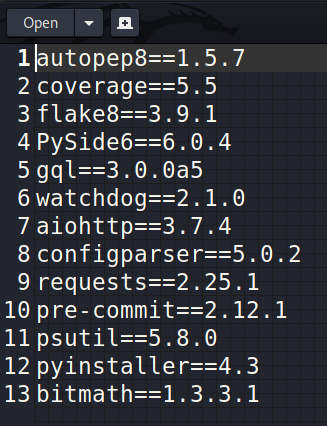
\includegraphics[scale = 0.5]{components/img/requirements.png}
    \caption{Struttura del file contenente le librerie}
    \label{fig:Struttura del file contentente le librerie}
\end{figure}
Per poter installare una nuova libreria il procedimento è semplice:
\begin{itemize}
	\item Aprire il file "\textit{requirements.txt}";
	\item Posizionarsi a fine file;
	\item Aggiungere una nuova riga;
	\item Aggiungere la nuova libreria.
\end{itemize}
La sintassi per l'aggiunta della libreria è la seguente:
\newline{} \centerline{\textbf{nome\_libreria==numero\_versione}}\newline{} 
\subsection{Struttura progetto}
Il progetto segue la seguente struttura:
\begin{figure}[H]
    \centering
    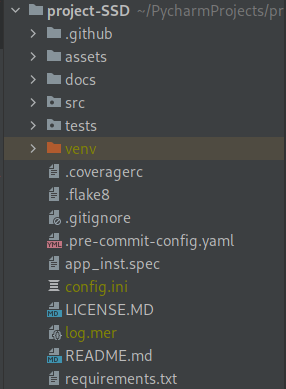
\includegraphics[scale = 0.5]{components/img/struttura-cartella-ssd.png}
    \caption{Struttura del progetto}
    \label{fig:Struttura del progetto}
\end{figure}  
\subsubsection{.github}
La cartella .github contiene tutte le informazioni necessarie per la \gloman{CI}. Essa è strutturata nel seguente modo:
\begin{figure}[H]
    \centering
    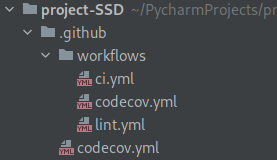
\includegraphics[scale = 0.5]{components/img/struttura-cartella-dotgithub.png}
    \caption{Struttura della cartella .github}
    \label{fig:Struttura della cartella .github}
\end{figure}
Il file "codecov.yml" posizionato dentro la cartella .github serve per poter impostare le regole generali per il controllo del valore della percentuale di test. Nella seguente tabella vengono riportate le \gloman{keyword} utilizzate con la loro descrizione:
{
	\setlength{\freewidth}{\dimexpr\textwidth-1\tabcolsep}
	\renewcommand{\arraystretch}{1.5}
	\setlength{\aboverulesep}{0pt}
	\setlength{\belowrulesep}{0pt}
	\rowcolors{2}{AzzurroGruppo!10}{white}
	\begin{longtable}{L{.15\freewidth} L{.60\freewidth}}
		\rowcolor{AzzurroGruppo!30}
		\textbf{Keyword} & \textbf{Descrizione}\\
		\toprule
		\endhead	
		Precision & La precisione delle cifre dopo la virgola della percentuale di codice coperto da test.\\
		Round & Come viene arrotondata la cifra dopo la troncatura determinata dalla precisione selezionata.\\
		Range & Il valore minimo e massimo della percentuale di codice coperto da test, valori esclusi da questo intervallo faranno fallire la \gloman{CI}. \\
		\bottomrule
		\hiderowcolors
		\caption{Parole chiave per file codecov.yml di configurazione generale}
	\end{longtable}
}
\begin{figure}[H]
    \centering
    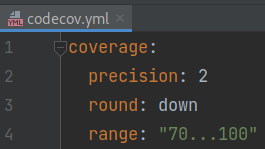
\includegraphics[scale = 0.5]{components/img/contenuto-github-codecov.png}
    \caption{Contenuto file codecov.yml}
    \label{fig:Contenuto file codecov.yml}
\end{figure}  
I file contenuti dentro la folder "workflows" invece specificano diverse regole per la configurazione della \gloman{CI}, meglio riassunte nella seguente tabella:
{
	\setlength{\freewidth}{\dimexpr\textwidth-1\tabcolsep}
	\renewcommand{\arraystretch}{1.5}
	\setlength{\aboverulesep}{0pt}
	\setlength{\belowrulesep}{0pt}
	\rowcolors{2}{AzzurroGruppo!10}{white}
	\begin{longtable}{L{.15\freewidth} L{.85\freewidth}}
		\rowcolor{AzzurroGruppo!30}
		\textbf{Keyword} & \textbf{Descrizione}\\
		\toprule
		\endhead	
		ci.yml & Configurazione delle \gloman{actions} di GitHub. Si ha una prima fase di setup dei vari sistemi operativi, vengono poi indicate le azioni che dovranno essere eseguite ed infine l'ultima azione comunica nell'apposito canale slack il successo della \gloman{CI}.\\
		codecov.yml & Configurazione della \gloman{CI} nel sito codecov che servirà a tenere traccia della percentuale di codice coperta da test.\\
		lint.yml & Configurazione dell'analisi statica che avverrà ad ogni commit. \\
		\bottomrule
		\hiderowcolors
		\caption{Nome e descrizione delle configurazioni per la CI}
	\end{longtable}
}
\subsubsection{assets}    
\begin{figure}[H]
    \centering
    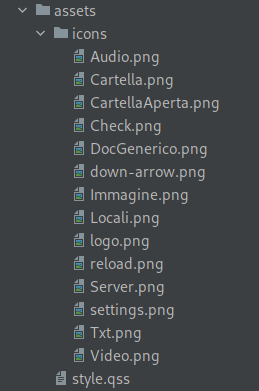
\includegraphics[scale = 0.5]{components/img/struttura-cartella-assets.png}
    \caption{Struttura della cartella assets}
    \label{fig:Struttura della cartella assets}
\end{figure}   
\subsubsection{docs}    
\begin{figure}[H]
    \centering
    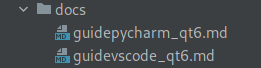
\includegraphics[scale = 0.5]{components/img/struttura-cartella-docs.png}
    \caption{Struttura della cartella docs}
    \label{fig:Struttura della cartella docs}
\end{figure}    
\subsubsection{src} \label{sec:cartelle-src}
\begin{figure}[H]
    \centering
    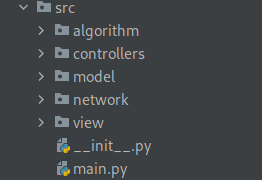
\includegraphics[scale = 0.5]{components/img/struttura-cartella-src.png}
    \caption{Struttura della cartella src}
    \label{fig:Struttura della cartella src}
\end{figure}    
\subsubsection{tests}    
\begin{figure}[H]
    \centering
    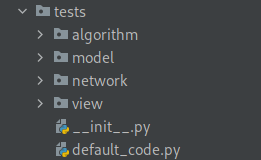
\includegraphics[scale = 0.5]{components/img/struttura-cartella-tests.png}
    \caption{Struttura della cartella tests}
    \label{fig:Struttura della cartella tests}
\end{figure}